\documentclass[12pt]{article}

\usepackage{amsmath}
\usepackage{graphicx}
\usepackage{booktabs}
\usepackage[a4paper, margin=1in]{geometry}

\title{Labwork 3: Logistic Regression}
\author{Nguyen Xuan Vinh}
\date{\today}

\begin{document}

\maketitle

\section{Introduction}

Logistic Regression is a supervised Machine Learning algorithm used for binary classification problems. 
Unlike Linear Regression, Logistic Regression predicts probabilities between 0 and 1 using the sigmoid activation function.

In this labwork, Logistic Regression was implemented completely from scratch using Gradient Descent optimization without using Machine Learning libraries such as NumPy, Scikit-learn, TensorFlow, or PyTorch.

The objective of this experiment is to predict loan approval decisions based on two features:
\begin{itemize}
    \item Experience
    \item Salary
\end{itemize}

The model optimizes three parameters:
\[
w_0,\ w_1,\ w_2
\]

using Gradient Descent.

\section{Mathematical Formulation}

The Logistic Regression model first computes a linear combination:

\[
z = w_1x_1 + w_2x_2 + w_0
\]

where:
\begin{itemize}
    \item \(x_1\) is Experience
    \item \(x_2\) is Salary
    \item \(w_1, w_2\) are weights
    \item \(w_0\) is the bias term
\end{itemize}

The sigmoid activation function is then applied:

\[
\sigma(z) = \frac{1}{1 + e^{-z}}
\]

The predicted probability is:

\[
\hat{y} = \sigma(z)
\]

The loss function used in this implementation is the squared error loss:

\[
L = \frac{1}{2}(\hat{y} - y)^2
\]

The Gradient Descent update rules are:

\[
w_0 = w_0 - r \frac{\partial L}{\partial w_0}
\]

\[
w_1 = w_1 - r \frac{\partial L}{\partial w_1}
\]

\[
w_2 = w_2 - r \frac{\partial L}{\partial w_2}
\]

where \(r\) is the learning rate.

\section{Algorithm Implementation}

The algorithm was implemented manually in Python.

The implementation process consists of the following steps:

\begin{enumerate}
    \item Read training data manually from the CSV file
    \item Initialize parameters \(w_0, w_1, w_2\)
    \item Compute the linear combination \(z\)
    \item Apply the sigmoid activation function
    \item Compute prediction loss
    \item Calculate gradients manually
    \item Update parameters using Gradient Descent
    \item Repeat iteratively until convergence
\end{enumerate}

The implementation does not use:
\begin{itemize}
    \item NumPy
    \item Scikit-learn
    \item Pandas
    \item TensorFlow
    \item PyTorch
\end{itemize}

Only basic Python and Matplotlib were used.

\section{Dataset}

The dataset used in this experiment is stored in the file \texttt{loan2.csv}.

The dataset contains:
\begin{itemize}
    \item Experience
    \item Salary
    \item Loan approval result
\end{itemize}

\begin{table}[h]
\centering
\begin{tabular}{ccc}
\toprule
Experience & Salary & Loan \\
\midrule
3 & 4 & 1 \\
2.5 & 4 & 1 \\
1 & 4 & 0 \\
2.5 & 5 & 1 \\
2 & 5 & 1 \\
1.5 & 5 & 0 \\
0.5 & 5 & 0 \\
1.75 & 6 & 1 \\
0.25 & 6 & 0 \\
1 & 7 & 1 \\
\bottomrule
\end{tabular}
\caption{Partial training dataset}
\end{table}

The dataset is relatively small and simple, making it suitable for understanding the behavior of Logistic Regression and Gradient Descent optimization.

\section{Experimental Results}

The model was trained using:
\[
learning\ rate = 0.001
\]

and:
\[
iterations = 2000
\]

The initial parameter values were:

\[
w_0 = 0,\quad w_1 = 0,\quad w_2 = 0
\]

\subsection{Intermediate Optimization Results}

Several intermediate training steps are shown below.

\begin{table}[h]
\centering
\begin{tabular}{ccccc}
\toprule
Step & Loss & \(w_0\) & \(w_1\) & \(w_2\) \\
\midrule
0 & 0.126197 & -0.000475 & 0.005558 & -0.003075 \\
500 & 0.078861 & -0.317198 & 1.215263 & -0.131204 \\
1000 & 0.073850 & -0.733791 & 1.540975 & -0.113094 \\
1500 & 0.069938 & -1.147225 & 1.701640 & -0.075163 \\
1900 & 0.067083 & -1.465464 & 1.788582 & -0.041643 \\
\bottomrule
\end{tabular}
\caption{Intermediate Gradient Descent optimization results}
\end{table}

The loss value decreases steadily during training:

\[
0.126197 \rightarrow 0.067083
\]

This indicates that the model successfully learns from the training data and improves prediction performance over time.

The final learned parameters are:

\[
w_0 = -1.542210
\]

\[
w_1 = 1.807181
\]

\[
w_2 = -0.033287
\]

The learned model suggests that experience has a strong positive influence on loan approval prediction.

\section{Prediction Results}

Several prediction examples produced by the trained model are shown below.

\begin{table}[h]
\centering
\begin{tabular}{cccc}
\toprule
Experience & Salary & Probability & Prediction \\
\midrule
3.0 & 4.0 & 0.9769 & 1 \\
0.5 & 5.0 & 0.3089 & 0 \\
1.75 & 6.0 & 0.8054 & 1 \\
0.25 & 7.0 & 0.2102 & 0 \\
2.0 & 8.0 & 0.8589 & 1 \\
\bottomrule
\end{tabular}
\caption{Sample Logistic Regression predictions}
\end{table}

The model correctly predicts most training samples based on the probability threshold of 0.5.

\section{Effect of Learning Rate}

The learning rate significantly affects convergence behavior.

\begin{itemize}
    \item Small learning rates produce slow but stable convergence
    \item Suitable learning rates improve optimization efficiency
    \item Large learning rates may cause unstable updates and divergence
\end{itemize}

In this experiment, the learning rate \(r = 0.001\) provides stable convergence and smooth reduction of the loss function.

\section{Loss Visualization}

Figure 1 shows the training loss during Gradient Descent optimization.

\begin{figure}[h]
\centering
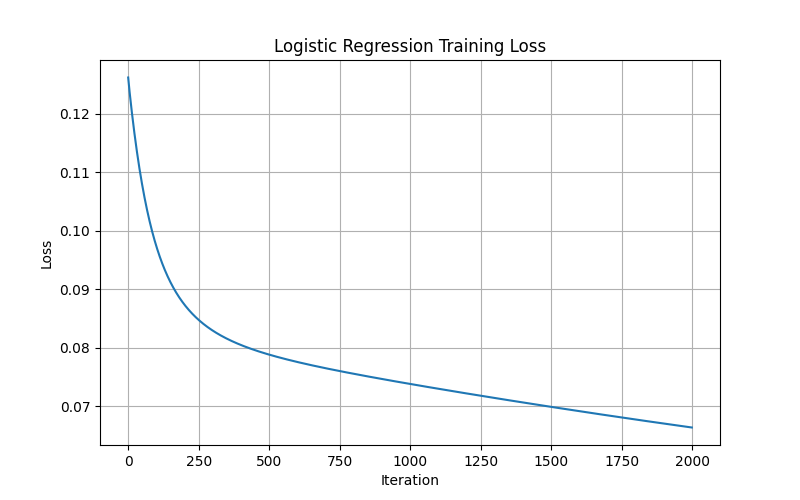
\includegraphics[width=0.8\textwidth]{loss.png}
\caption{Training loss versus iteration}
\end{figure}

The graph shows that the loss decreases progressively as training continues, demonstrating successful optimization.

\section{Discussion}

The experiments demonstrate that Logistic Regression can successfully solve binary classification problems using Gradient Descent optimization.

As training progresses:
\begin{itemize}
    \item The loss decreases steadily
    \item Prediction probabilities become more accurate
    \item The model learns decision boundaries from the dataset
\end{itemize}

Although the dataset is relatively small, the implementation provides practical understanding of:
\begin{itemize}
    \item Logistic Regression
    \item Sigmoid activation
    \item Binary classification
    \item Gradient Descent optimization
\end{itemize}

\section{Conclusion}

In this labwork, Logistic Regression was successfully implemented completely from scratch using Python.

The implementation:
\begin{itemize}
    \item Reads data manually from a CSV file
    \item Computes sigmoid predictions
    \item Optimizes parameters using Gradient Descent
    \item Prints intermediate optimization results
    \item Generates visualization of training loss
\end{itemize}

The experimental results show that the model successfully learns patterns from the dataset and performs binary classification effectively.

This labwork provides practical understanding of optimization and classification techniques commonly used in Machine Learning and Deep Learning.

\end{document}